\lecture{2009-11-18}
%
\noindent weitere Darstellung von $\euler$:
\begin{equation*}
  \euler = \liminfty{\left(1+\frac 1 n\right)^n}\text{ (langsam konvergent)}
\end{equation*}
%
Weg zur Einführung der $\euler$-Funktion:
\begin{equation*}
  \text{z. z.} \forall x \in \mathbb{R}\; \left( 1 + \frac x n \right)^n \text{ konvergent}
\end{equation*}
Beweis siehe \cite[S. 32]{bornemann}

\begin{note}
  Bisher wurde in allen Definitionen und Erläuterungen Kenntnis eines Grenzwerts vorausgesetzt.\\
  Frage: Reichen Folgenelemente eventuell aus?\\
  Antwort: Cauchy'sche Folge
\end{note}

\begin{definition}[Cauchy-Folge]
  Die Folge $a_n$ heißt Cauchy-Folge, falls
  \[ \forall \varepsilon > 0\; \exists N(\varepsilon)\; \forall n,m \geq N: \left| a_n-a_m \right| < \varepsilon \]
\end{definition}

\begin{proposition}
  $a_n$ konvergent $\Leftrightarrow$ $a_n$ ist Cauchyfolge
\end{proposition}

\begin{proof}
  \begin{itemize}
    \item[$(\Rightarrow)$]
      \begin{align*}
        \left| a_n - a_m \right| &= \left| a_n - \alpha + \alpha - a_m \right| \text{ (Grenzwert $\alpha$ existiert)}\\
        &\leq \left| a_n - \alpha\right| + \left| a_m - \alpha \right|, \text{ mit $n,m \geq N(\varepsilon)$}\\
        &<\varepsilon+\varepsilon = 2\varepsilon
        \intertext{setze $\overline N (\varepsilon) = N\left(\frac \varepsilon 2\right)$, damit}
        \left| a_n - a_m \right| &< \varepsilon
      \end{align*}
        %< \varepsilon$
    \item[$(\Leftarrow)$] 1780-1860\\
      Beweisidee:
      \begin{itemize}
        \item Beschränktheit der Cauchy-Folge
        \item $\frac 1 n, 1+\frac 1 n, 2+\frac 1 n, \frac 2 n, 1+\frac 2 n, 2+\frac 2 n, \ldots$
              \annotation{abwechselnd die Folgeglieder der Folgen $\frac 1 n$, $1+\frac 1 n$ und $2+\frac 1 n$}\\
              mehrere Kandidaten für Grenzwerte -- Häufungspunkte
              \annotation{Häufungspunkt wird ähnlich wie der Grenzwert definiert; jedoch brauchen nicht \emph{alle}, sondern nur \emph{unendlich viele} Folgeglieder in der $\varepsilon$-Umgebung liegen}
        \item Teilfolge, die gegen den Häufungspunkt konvergiert
        \item Bolzano-Weierstraß: Jede beschränkte Folge besitzt mindestens einen Häufungspunkt; eine konvergente Teilfolge ist auswählbar
        \item eindeutiger Grenzwert für Cauchy-Folge $\limsup$ bzw. $\liminf$
        \item Beweis siehe \cite[S. 29ff]{bornemann}
      \end{itemize}
  \end{itemize}
\end{proof}

\subsection{Stetige Funktionen}

Idee: Übertrage Grenzwerte im Definitionsbereich auf den Wertebereich\\
"`gutmütige"' Funktionen $f: I \to \mathbb{R}$, die einen Grenzprozess übertragen

\subsubsection*{formal}
\begin{equation*}
  \left.
  \begin{matrix}[rll]
    \text{linksseitiger Grenzwert} & x \longrightarrow a^+ & \displaystyle\lim_{x \rightarrow a^+} f(x) = c \\*[5mm]
    \text{rechtsseitiger Grenzwert} & x \longrightarrow a^- & \displaystyle\lim_{x \rightarrow a^-} f(x) = c
  \end{matrix}
  \right\}\implies \text{stetig}
\end{equation*}

\begin{definition}[Stetigkeit]
  $f: I \to \mathbb{R}$ heißt stetig in $x_0 \in I$, falls \begin{equation*} \lim_{x\rightarrow x_0} f(x) = f(x_0). \end{equation*} (alle denkbaren Folgen, die gegen $x_0$ konvergieren, sind zugelassen)

  $f$ heißt stetig, falls $f$ stetig in allen $x_0 \in I$ ist.
\end{definition}

\subsubsection*{anschaulich}
"`Zeichnen ohne den Stift abzusetzen"'

\begin{center}
\begin{tikzpicture}[]
 \draw[->,semithick] (-3,0) -- (3,0);
 \draw (-2,0.15) -- (-2,-0.15) node[below] {$a$};
 \draw (2,0.15) -- (2,-0.15) node[below] {$b$};
 \draw[domain=-2:2] plot [id=stetig_a, samples=50] function {0.1*(x**3)+1};
 \node at (0,1.7) {$f(x)$};
\end{tikzpicture}

\begin{tikzpicture}[]
 \draw[->,semithick] (-3,0) -- (3,0);
 \draw (-2,0.2) -- (-2,-0.2) node[below] {$a$};
 \draw (2,0.2) -- (2,-0.2) node[below] {$b$};
 \draw (-2,1) -- (-1.7,0.7) -- (-1.5,2.2) -- (-1.1,0.3) -- (0,1.3) -- (0.7,0.7) -- (1.2,3) -- (2,0.5);
 \node at (0,1.7) {$f(x)$};
 \node at (4,2) {"`Ecken erlaubt"'};
\end{tikzpicture}
\end{center}

\begin{figure}[h]\centering

  \subfloat[Sprünge]{
  
\begin{tikzpicture}[]
 \draw[->,semithick] (-0.5,0) -- (3.5,0);
 \draw [)-|] (0,1) -- (1,1);
 \draw [)-|] (1,2) -- (2,2);
 \draw [)-|] (2,3) -- (3,3);
 %\node at (0,-1) {Sprünge};
\end{tikzpicture}
  }
  \subfloat[Lücken]{
\begin{tikzpicture}[]
 \draw[->,semithick] (-2.3,0) -- (2.3,0);
 \draw[domain=-2:0] plot [id=stetig_b1, samples=50] function {0.1*(x**3)+1};
 \draw[domain=0.5:2] plot [id=stetig_b2, samples=50] function {0.1*(x**3)+1.2};
 %\node at (0,-1) {Lücken};
\end{tikzpicture}
  }
  \subfloat[Polstellen]{
\begin{tikzpicture}[]
 \draw[->,semithick] (-2.3,0) -- (2.3,0);
 \draw (0,0.2) -- (0,-0.2) node[below] {$0$};
 \draw[domain=-2:-1.05] plot [id=stetig_c1, samples=30] function {(0.1*x)/((x+1)*(x-1))};
 \draw [ dashed](-1,1) -- (-1,-1);
 \draw[domain=-0.95:0.95] plot [id=stetig_c2, samples=30] function {(0.1*x)/((x+1)*(x-1))};
 \draw [ dashed](1,1) -- (1,-1);
 \draw[domain=1.05:2] plot [id=stetig_c3, samples=30] function {(0.1*x)/((x+1)*(x-1))};
 %\node at (0,-1) {Polstellen};
\end{tikzpicture}
  }
  \caption{Unstetigkeiten}
\end{figure}


\begin{theorem}[$\delta$-$\epsilon$-Charakterisierung analog zur Folgenkonvergenz]\label{thm:delta_epsilon}
  Für $f: I \to \mathbb{R}, x_0 \in I$ sind äquivalent:
  \begin{enumerate}
    \item $f$ stetig in $x_0$ (d. h. $\displaystyle\lim_{x\rightarrow x_0} f(x) = f(x_0)$)
    \item
      \begin{equation*}
        \forall \varepsilon > 0\; \exists \delta > 0\; \forall x \in I\; \left(
          \underbrace{\left| x-x_0\right| < \delta}_{\text{Definitionsbereich}} \implies
          \underbrace{\left| f(x)-f(x_0)\right| < \epsilon}_{\text{Wertebereich}}
        \right)
      \end{equation*}
  \end{enumerate}
\end{theorem}

\begin{center}
\begin{tikzpicture}[]
 \draw[->,semithick] (-0.5,0) -- (3,0) node[below]{x};
 \draw[->,semithick] (0,-0.5) -- (0,2.5) node[left]{y};
 \draw (1,0.2) -- (1,-0.2) node[below] {$x_0$};
 \draw (0.2,1) -- (-0.2,1) node[left] {$f(x_0)$};
 \draw [dashed] (0,1) -- (1,1) -- (1,0);
 \draw [dashed] (0,1.1) -- (1.55,1.1) -- (1.55,0);
 \draw [dashed] (0,0.9) -- (0.45,0.9) -- (0.45,0);
 \draw[domain=0:2.2] plot [id=stetig_d, samples=50] function {0.6*((x-1)**3)+1};
 \draw [|<->|] (2,1.1) -- (2,0.9) node [right] {\footnotesize $2\varepsilon$};
 \draw [|<->|] (1.55,-0.7) -- (0.45,-0.7) node[below right] {$\;\;2\delta$};
\end{tikzpicture}
\end{center}



\begin{example}
  \begin{itemize}
    \item $\sin\left(\frac 1 x\right)$: unstetig
    \begin{center}
      \begin{tikzpicture}
        \draw[->,semithick] (-2.1,0) -- (2.1,0) node[below]{x};
        \draw[->,semithick] (0,-1.1) -- (0,1.1) node[left]{y};
        \draw[domain=-2:2] plot [id=sin_a, samples=400] function {sin(1/x)};
      \end{tikzpicture}
    \end{center}

    \item $x \cdot \sin\left(\frac 1 x\right)$: stetig ergänzbar an der Stelle $0$, da Nullfolge $\cdot$ beschränkte Folge = Nullfolge (siehe Rechenregeln auf Seite \pageref{ssub:nullfolgen})
    \begin{center}
      \begin{tikzpicture}
        \draw[->,semithick] (-2.1,0) -- (2.1,0) node[below]{x};
        \draw[->,semithick] (0,-1.1) -- (0,1.1) node[left]{y};
        \draw[domain=-2:2] plot [id=sin_b, samples=400] function {x*sin(1/x)};
      \end{tikzpicture}
    \end{center}
  \end{itemize}
\end{example}

\subsubsection*{Rechenregeln stetiger Funktionen}

$f, g: I \to \mathbb{R}$ stetig

\begin{enumerate}
  \item $f\pm g$ stetig
  \item $\alpha \in \mathbb{R}$: $\alpha \cdot f$ stetig
  \item $f \cdot g$ stetig (Produkt der Funktionswerte)
  \item $g(x) \neq 0$: $\frac f g$ stetig
  \item Komposition/Hintereinanderausführung
    \begin{equation*}
      g(I) \subseteq I: \qquad (f \circ g)(x) = f(g(x)) \text{ stetig}
    \end{equation*}
\end{enumerate}
%
Beweise per $\delta-\epsilon$-Charakterisierung, siehe \cite{bornemann}

\subsubsection*{Folgerungen}

  \begin{enumerate}
    \item jedes Polynom $p(x) = a_0 + a_1 x + \ldots + a_n x^n$ ist stetig\\
      Argumentation:
      \begin{itemize}
        \item[] $f(x) = x$ stetig
        \item[$\implies$] $x^2, \ldots, x^k$ stetig
        \item[$\implies$] $a_k x^k, \ldots, a_1 x$ stetig
        \item[$\implies$] Summe stetig
      \end{itemize}
    \item jede rationale Funktion $r(x) = \frac{p(x)}{q(x)}$ ist bis auf Nullstellen im Nenner stetig
  \end{enumerate}

\subsubsection*{Eigenschaften stetiger Funktionen}

$f$ stetig auf dem Intervall $\left[a,b\right]$
  \begin{enumerate}
    \item $f$ ist beschränkt
      \begin{note}
        Zentral hierbei ist, dass es sich um ein abgeschlossenes Intervall handeln muss.

        Bsp.: $f(x) = \frac 1 x$, halboffenes Intervall $\left]0,1\right]$, $\displaystyle\lim_{x\rightarrow 0^+} = \infty$ $\implies$ Polstelle $\implies$ nicht beschränkt
      \end{note}
    \item $f$ nimmt Minimum/Maximum in diesem Intervall an (Extremwertsatz)
    \item falls $f(a) < 0$ und $f(b) > 0$, dann existiert ein $x^\ast$ mit $f(x^\ast) = 0$ (Zwischenwertsatz)
    
      (Beweis per Bisektionsverfahren, Intervallhalbierung)
  \end{enumerate}
\begin{center}
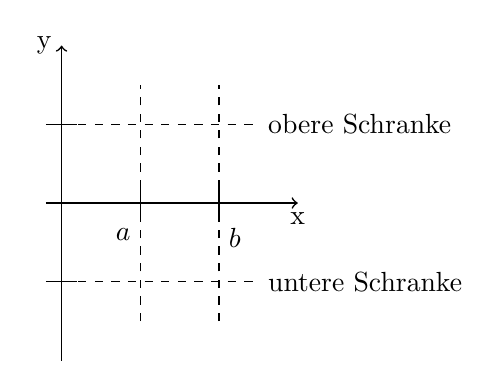
\begin{tikzpicture}
 \draw[->,semithick] (-0.2,0) -- (3,0) node[below]{x};
 \draw[->,semithick] (0,-2) -- (0,2) node[left]{y};
 \draw (1,0.2) -- (1,-0.2) node[below left] {$a$};
 \draw (2,0.2) -- (2,-0.2) node[below right] {$b$};
 \draw (-0.2,1) -- (0.2,1);
 \draw (-0.2,-1) -- (0.2,-1);
 \draw [dashed] (0,1) -- (2.5,1) node[right] {obere Schranke};
 \draw [dashed] (0,-1) -- (2.5,-1) node[right] {untere Schranke};
 \draw [dashed] (1,-1.5) -- (1,1.5);
 \draw [dashed] (2,-1.5) -- (2,1.5);
 \draw[domain=1:2] plot [id=sin_b, samples=400] function {sin(6*(x-0.5))};
\end{tikzpicture}
\end{center}

